\chapter{Introduction}

\section{Anchor Placement: Equal distribution along 45 Degree Axis}
For the first round of testing, chosen more as an excercise in the simulation analysis package in MATLAB\copyright, 4 anchor nodes are placed at the closest node the the 45-degree axes, with increasing distance from the center. \ref{fig:45DegreeAxisRandomNetwork} shows the positions for each iteration. 

\begin{figure}
  % Requires \usepackage{graphicx}
  \centering
  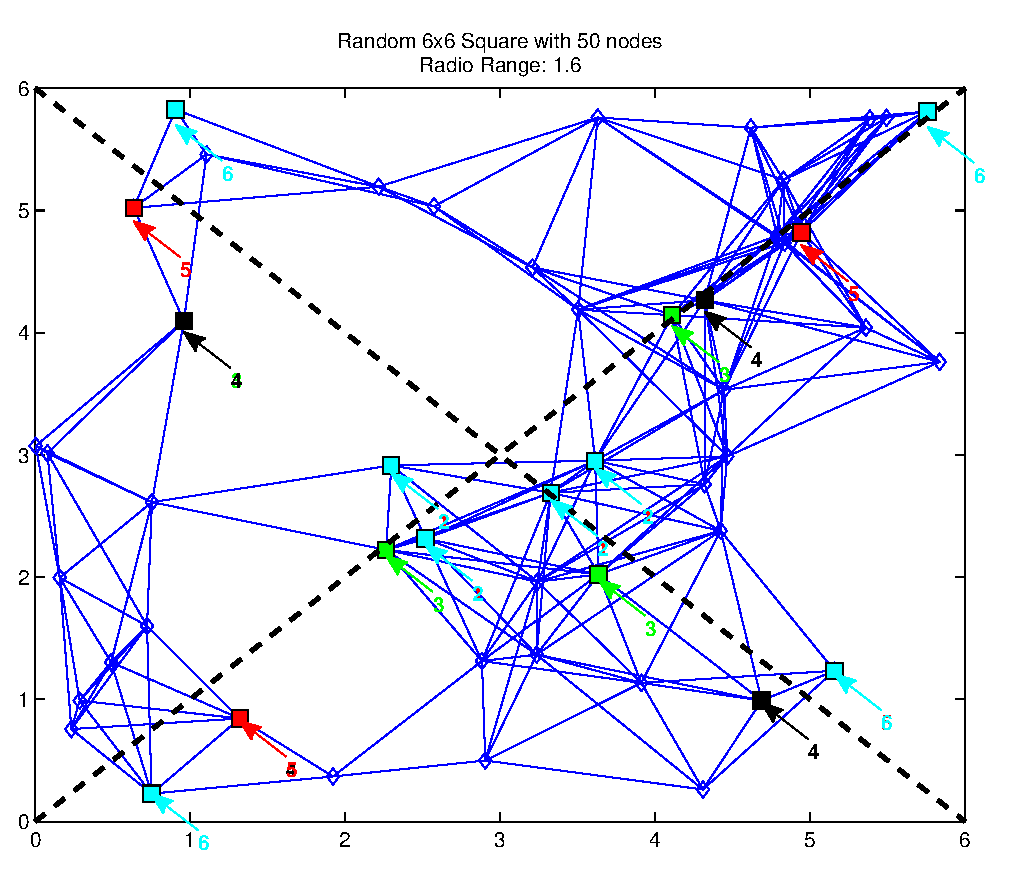
\includegraphics[width=4in]{../cca/results/45DegreeAxis_Random/networkRandom6x6Squarewith50nodes1-6Radius.eps}\\
  \caption{The random network used, showing the 6 position sets of anchors.}
  \label{fig:45DegreeAxisRandomNetwork}
\end{figure}

The 2nd graph in \ref{fig:45DegreeAxisRandomResults} shows that the best localization performance is achieved when the 4 anchors are roughly midway between the center of the network and the corners.  

\begin{figure}
    \centerline{
      \subfigure[Error decreasing as network connectivity increases]
      {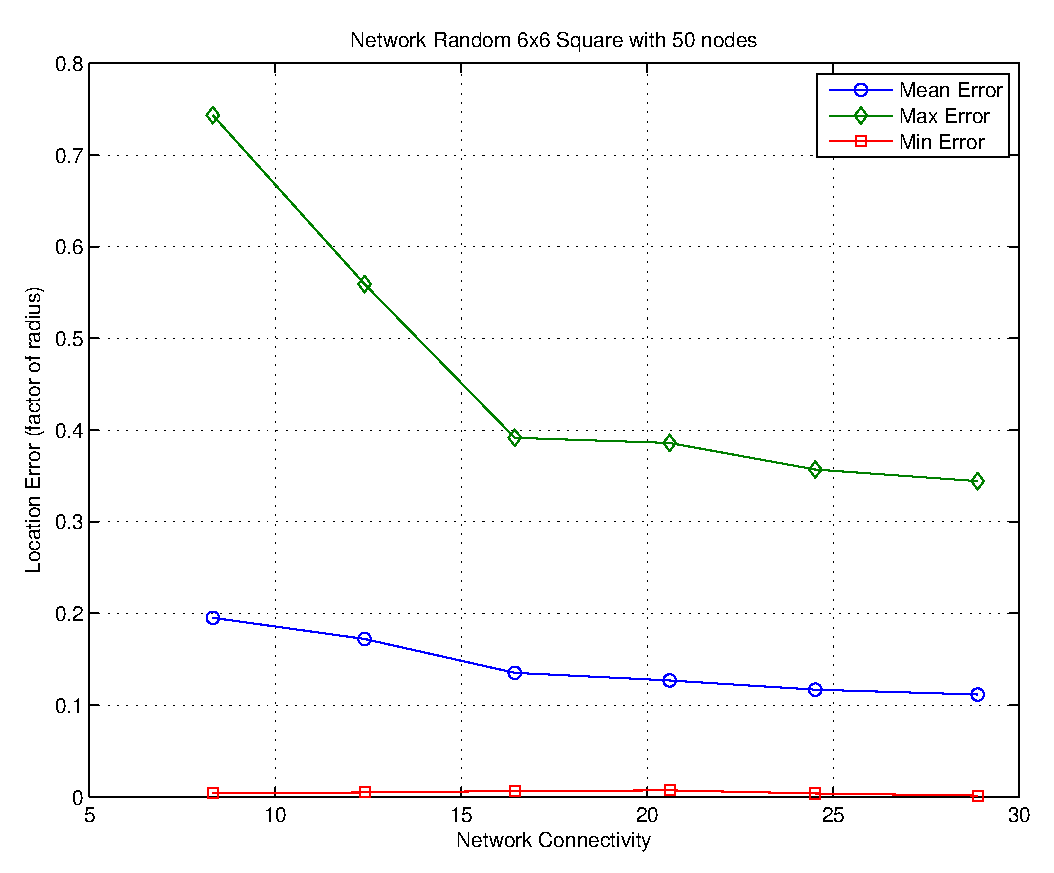
\includegraphics[width=2.5in]{../cca/results/45DegreeAxis_Random/NetworkConn-vs-Error-Random-6x6-Square-with-50-nodes-1.6-to-3.4radius-50.eps}}\hfil
      \subfigure[Error is lowest as the anchors are near the midpoint between center and corners]
      {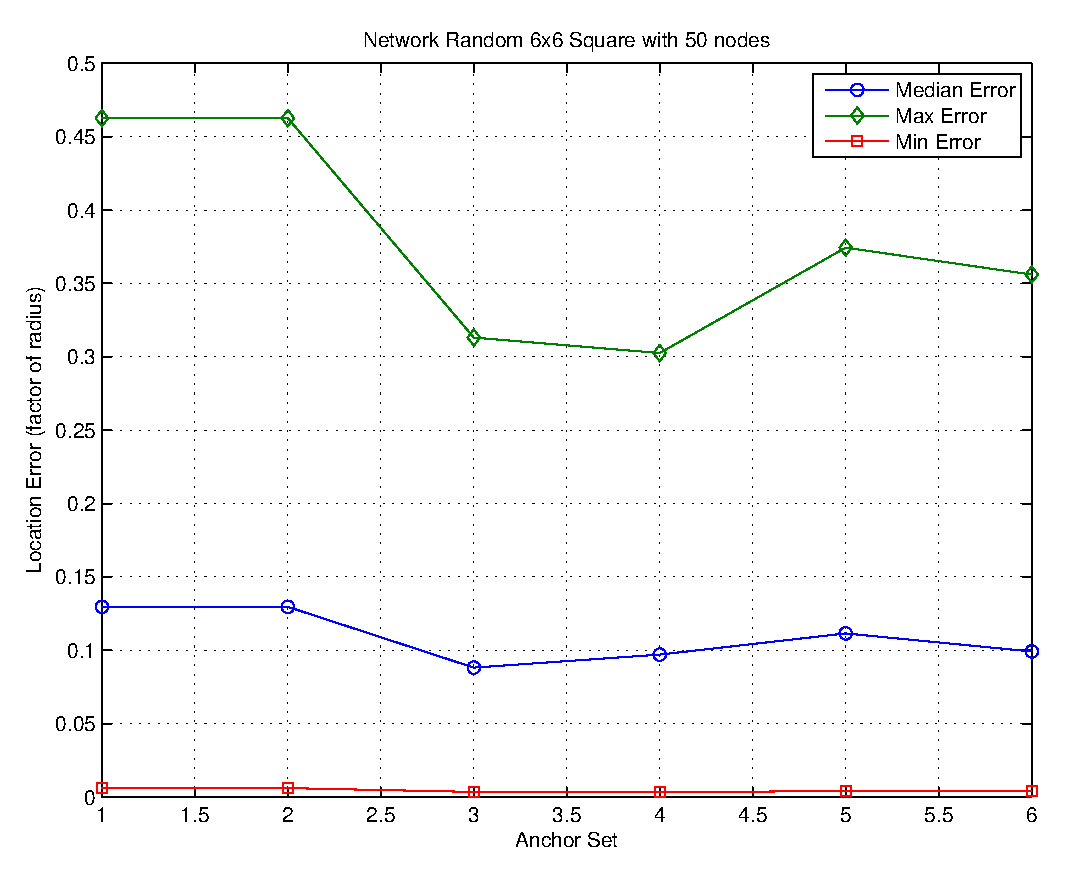
\includegraphics[width=2.5in]{../cca/results/45DegreeAxis_Random/AnchorSets-vs-Error-Random-6x6-Square-with-50-nodes-1.6-to-3.4radius-50.eps}} }
    \caption{Maximum, median, and minimum errors for various network conditions} \label{fig:45DegreeAxisRandomResults}
\end{figure}

The same test is repeated for a grid network layout instead of a random network layout.

\begin{figure}
  % Requires \usepackage{graphicx}
  \centering
  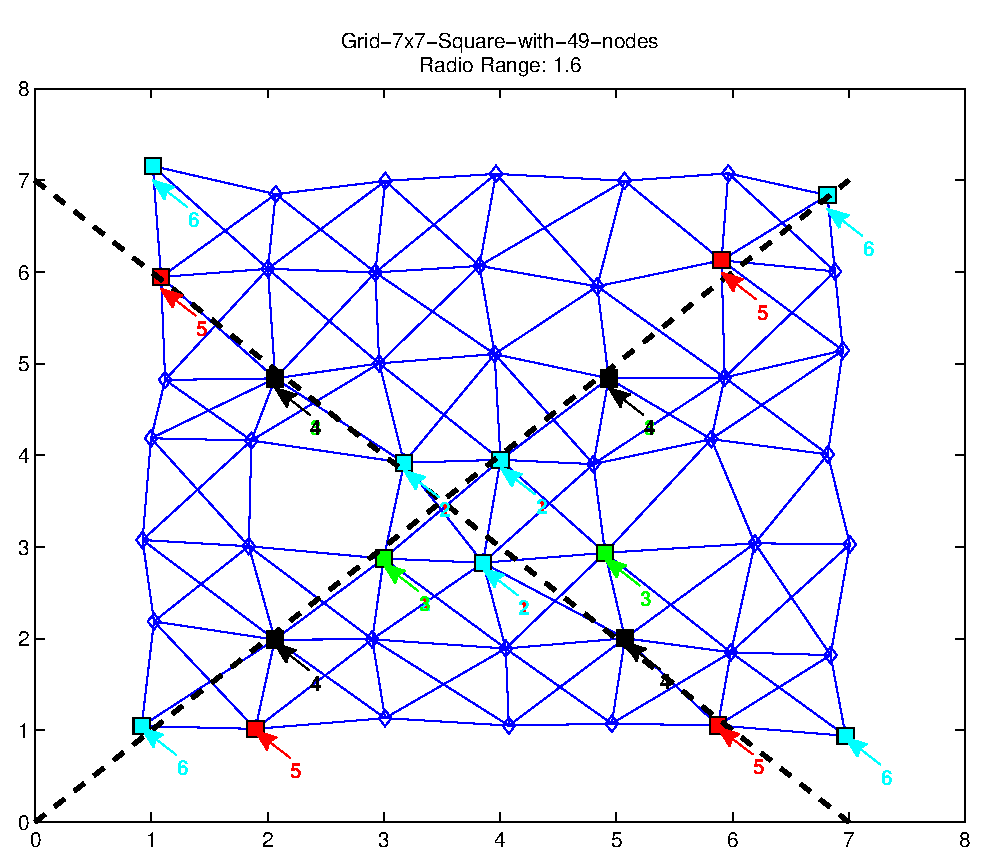
\includegraphics[width=4in]{../cca/results/45DegreeAxis_Grid/network-Grid-7x7-Square-with-49-nodes-Radius1.6.eps}\\
  \caption{The random network used, showing the 6 position sets of anchors.}
  \label{fig:45DegreeAxisGridNetwork}
\end{figure}


\begin{figure}
    \centerline{
      \subfigure[Error decreasing as network connectivity increases]
      {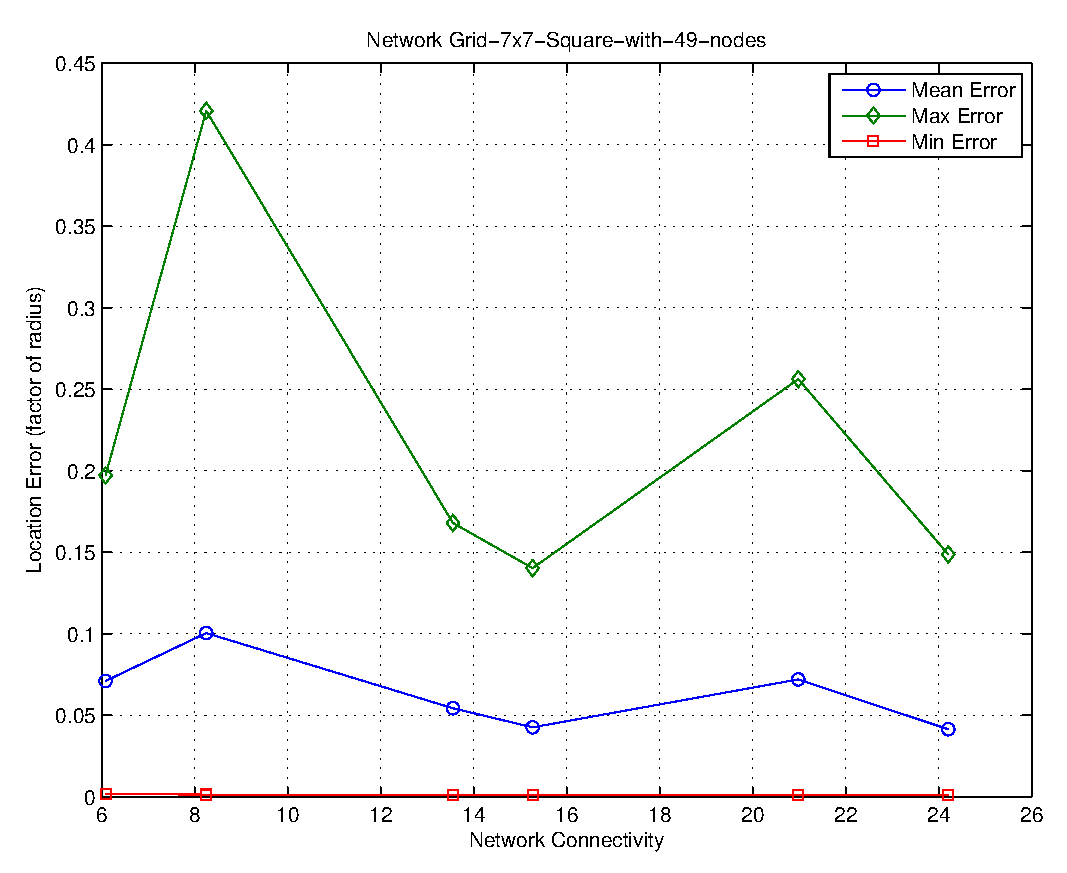
\includegraphics[width=2.5in]{../cca/results/45DegreeAxis_Grid/Connectivity-vs-Error-Grid-7x7-Square-with-49-nodes-1.6-to-3.4Radius.eps}}\hfil
      \subfigure[Error is lowest as the anchors are near the midpoint between center and corners]
      {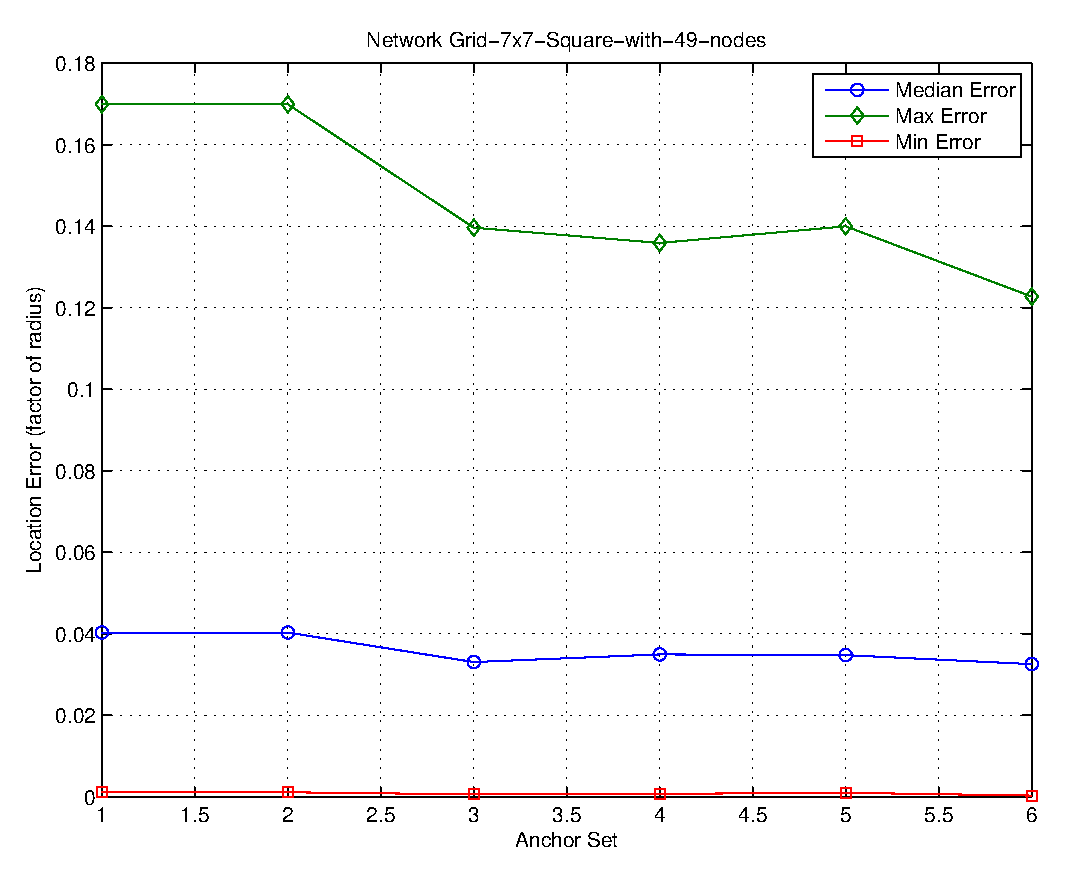
\includegraphics[width=2.5in]{../cca/results/45DegreeAxis_Grid/AnchorSetsVsError-Grid-7x7-Square-with-49-nodes-1.6-to-3.4Radius.eps}} }
    \caption{Maximum, median, and minimum errors for various network conditions} \label{fig:45DegreeAxisGridResults}
\end{figure}


% Above-below subfigure
%\begin{figure}
%    \centerline{ \subfigure[Case I]{
\includegraphics[width=2.5in]{CUlogo.jpg}} }
%    \centerline{ \subfigure[Case II]{
\includegraphics[width=2.5in]{MAElogo.jpg}} }
%    \caption{Samble above-below subfigures} \label{fig:above-below}
%\end{figure}

%\section{Section Demonstrating Tables}
%First paragraph.  This is a sample reference to Table
%\ref{tab:sample}.

%\begin{table}
%  \centering
%  \caption{Sample table. With an extra long caption to test how captions will wrap.}\label{tab:sample}
%    \vspace{6pt} % Required to get proper spacing between caption and table
%  \begin{tabular}{c c c}
%    \hline
%    Label 1 & Label 2 & Label 3 \\
%    \hline\hline
%    value 1 & $x_1$ & $y_1$ \\
%    value 2 & $x_2$ & $y_2$ \\
%    value 3 & $x_3$ & $y_3$ \\
%    \hline
%  \end{tabular}
%\end{table}

%New paragraph.

%\begin{equation}\label{eqn:newton_law}
%    F = Ma
%\end{equation}

%Paragraph referencing an equation \ref{eqn:newton_law}.
